\documentclass[12pt]{beamer}
\usepackage{../Estilos/BeamerMAF}
%Sección para el tema de beamer, con el theme, usercolortheme y sección de footers
\usetheme{CambridgeUS}
\usecolortheme{beaver}
%\useoutertheme{default}
\setbeamercovered{invisible}
% or whatever (possibly just delete it)
\setbeamertemplate{section in toc}[sections numbered]
\setbeamertemplate{subsection in toc}[subsections numbered]
\setbeamertemplate{subsection in toc}{\leavevmode\leftskip=3.2em\rlap{\hskip-2em\inserttocsectionnumber.\inserttocsubsectionnumber}\inserttocsubsection\par}
\setbeamercolor{section in toc}{fg=blue}
\setbeamercolor{subsection in toc}{fg=blue}
\setbeamercolor{frametitle}{fg=blue}
\setbeamertemplate{caption}[numbered]

\setbeamertemplate{footline}
\beamertemplatenavigationsymbolsempty
\setbeamertemplate{headline}{}


\makeatletter
\setbeamercolor{section in foot}{bg=gray!30, fg=black!90!orange}
\setbeamercolor{subsection in foot}{bg=blue!30!yellow, fg=red}
\setbeamercolor{date in foot}{bg=black, fg=white}
\setbeamertemplate{footline}
{
  \leavevmode%
  \hbox{%
  \begin{beamercolorbox}[wd=.333333\paperwidth,ht=2.25ex,dp=1ex,center]{section in foot}%
    \usebeamerfont{section in foot} \insertsection
  \end{beamercolorbox}%
  \begin{beamercolorbox}[wd=.333333\paperwidth,ht=2.25ex,dp=1ex,center]{subsection in foot}%
    \usebeamerfont{subsection in foot}  \insertsubsection
  \end{beamercolorbox}%
  \begin{beamercolorbox}[wd=.333333\paperwidth,ht=2.25ex,dp=1ex,right]{date in head/foot}%
    \usebeamerfont{date in head/foot} \insertshortdate{} \hspace*{2em}
    \insertframenumber{} / \inserttotalframenumber \hspace*{2ex} 
  \end{beamercolorbox}}%
  \vskip0pt%
}
\makeatother\newlength{\depthofsumsign}
\setlength{\depthofsumsign}{\depthof{$\sum$}}
\newcommand{\nsum}[1][1.4]{% only for \displaystyle
    \mathop{%
        \raisebox
            {-#1\depthofsumsign+1\depthofsumsign}
            {\scalebox
                {#1}
                {$\displaystyle\sum$}%
            }
    }
}
\def\scaleint#1{\vcenter{\hbox{\scaleto[3ex]{\displaystyle\int}{#1}}}}
\def\bs{\mkern-12mu}





\date{}
\title{Ecuación de Laplace en esferas \\ \large{Polinomios de Legendre}}
\author{M. en C. Gustavo Contreras Mayén}
\begin{document}
\maketitle
\fontsize{14}{14}\selectfont
\spanishdecimal{.}


\section*{Contenido}
\frame[allowframebreaks]{\tableofcontents[currentsection, hideallsubsections]}

%Ref. Hassani (2015)
\section{Problema a resolver}
\frame{\tableofcontents[currentsection, hideothersubsections]}
\subsection{Semiesferas a distintas temperaturas}

\begin{frame}
\frametitle{Enunciado}
Dos hemisferios sólidos conductores de calor de radio $a$, separados por un pequeño espacio aislante, forman una esfera. Las dos mitades de la esfera están en contacto, en el exterior, con dos baños de calor (infinitos) a temperaturas $T_{0}$ y $-T_{0} $, ver la figura (\ref{fig:figura_esfera_01}):
\end{frame}
\begin{frame}\label{figura_esferas}
\frametitle{Gráfica del problema a resolver}
\begin{figure}[H]
    \centering
    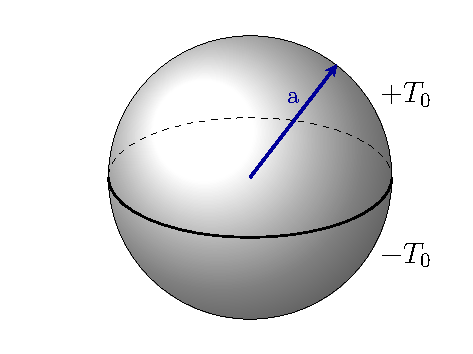
\includegraphics[scale=0.95]{Imagenes/Ejemplo_Esfera_01.eps}
    \caption{Dos hemisferios a distintas temperaturas.}
    \label{fig:figura_esfera_01}
\end{figure}
\hyperlink{llama_figura_esferas}{\beamerbutton{link}}
\end{frame}
\begin{frame}
\frametitle{Problema a resolver}
\textbf{Queremos encontrar la distribución de temperatura $T(r, \theta, \varphi)$ dentro de la esfera.}
\end{frame}

\section{Ecuación de Laplace}
\frame{\tableofcontents[currentsection, hideothersubsections]}
\subsection{Coordenadas esféricas}

\begin{frame}
\frametitle{Consideración de la geometría}
Dada la simetría esférica del problema, es directa la relación de trabajo con un sistema coordenado esférico $(r, \theta, \varphi)$.
\\
\bigskip
\pause
Tomando la ecuación de Laplace como punto de partida, habrá que expresarla en las coordenadas esféricas.
\end{frame}
\begin{frame}
\frametitle{Ecuación trasformada}
Como ya sabemos hacer el cambio entre el sistema cartesiano y el esférico, la ecuación de Laplace se expresa como:
\begin{align}
\begin{aligned}[b]
\dfrac{1}{r^{2}} \pdv{r} \left( r^{2} \pdv{\Psi}{r} \right) &+ \dfrac{1}{r^{2} \, \sin \theta} \bigg[ \pdv{\theta} \left( \sin \theta \pdv{\Psi}{\theta} \right) + \\[1em]
&+ \dfrac{1}{\sin \theta} \, \pdv[2]{\Psi}{\varphi} \bigg] = 0
\end{aligned}
\label{eq:ecuacion_22_15}
\end{align}
\end{frame}

\subsection{Separación de variables}

\begin{frame}
\frametitle{Simplificando la EDP2}
Para ocupar la técnica de separación de variables, proponemos una solución del tipo:
\pause
\begin{align*}
\Psi(r, \theta, \varphi) = R(r) \Theta (\theta) \Phi(\varphi)
\end{align*}
\pause
Que sustituimos en la ec (\ref{eq:ecuacion_22_15}).
\end{frame}
\begin{frame}
\frametitle{Haciendo el trabajo algebraico}
En el necesario paso de separar la ecuación en expresiones que dependan de una sola variable, en nuestro caso abreviamos el desarrollo.
\\
\bigskip
\pause
Pero en el camino encontramos \emph{dos constantes de separación}: $\alpha$ y $\beta$.
\end{frame}
\begin{frame}
\frametitle{Ecuaciones diferenciales ordinarias}
Tendremos tres ecuaciones diferenciales ordinarias, mucho más fácil de resolver que la ecuación diferencial parcial:
\end{frame}
\begin{frame}
\frametitle{Ecuación radial}
La ED02OH que depende solo de la variable $r$ es:
\pause
\begin{align}
\dfrac{1}{r^{2}} \dv{r} \left( r^{2} \dv{R}{r} \right) - \dfrac{\alpha}{r^{2}} R = 0
\label{eq:ecuacion_26_1a}
\end{align}
que es la \textbf{ecuación radial}.
\end{frame}
\begin{frame}
\frametitle{Ecuación polar}
La ecuación que depende solo de $\theta$ es:
\pause
\begin{align}
\dfrac{1}{\sin \theta} \dv{\theta} \left( \sin \theta \dv{\Theta}{\theta} \right) + \left( \alpha - \dfrac{\beta}{\sin^{2} \theta} \right) \Theta = 0
\label{eq:ecuacion_26_1b}
\end{align}
esta es la \textbf{ecuación polar}.
\end{frame}
\begin{frame}
\frametitle{Ecuación azimutal}
La ecuación que depende del ángulo azimutal $\varphi$, es:
\begin{align}
\dv[2]{\Phi}{\varphi} + \beta \Phi = 0
\label{eq:ecuacion_26_1c}
\end{align}
es la llamada \textbf{ecuación azimutal.}
\pause
Con esta ecuación haremos una importante consideración en la siguiente diapositiva.
\end{frame}
\begin{frame}
\frametitle{Problemas con simetría azimutal}
En casos donde sea conocido de antemano que el potencial sea independiente del ángulo azimutal $\varphi$, entonces el problema presenta una \textbf{simetría azimutal}.
\end{frame}
\begin{frame}
\frametitle{Consecuencia de la simetría azimutal}
En este caso, podemos suponer que se tiene una función constante $S$, tal que:
\begin{align*}
\dv[2]{S}{\varphi} + \beta S = 0
\end{align*}
\pause
Esto implica que $\beta = 0$, ya que $S$ es una función contante no nula.
\end{frame}
\begin{frame}
\frametitle{Ecuaciones resultantes}
Dejando el sistema de EDO2H reducido a dos expresiones:
\begin{align}
\begin{aligned}
\dfrac{1}{r^{2}} \dv{r} \left( r^{2} \dv{R}{r} \right) - \dfrac{\alpha}{r^{2}} R &= 0 \\[1em]
\dfrac{1}{\sin \theta} \dv{\theta} \left( \sin \theta \dv{\Theta}{\theta} \right) + \alpha \Theta &= 0
\end{aligned}
\label{eq:ecuacion_26_02}
\end{align}
\end{frame}

\section{Resolviendo las EDO2H}
\frame{\tableofcontents[currentsection, hideothersubsections]}
\subsection{Ecuación polar}

\begin{frame}
\frametitle{Recuperando las soluciones}
De manera inicial nos enfocamos en la ecuación polar.
\\
\bigskip
\pause
La presencia en el denominador del término $\sin \theta \dd{\theta}$ (que es el diferencial de $\cos \theta)$ sugiere el cambio de variable de $\theta$ a $u \equiv \cos \theta$.
\end{frame}
\begin{frame}
\frametitle{Cambiando la variable}
Para cualquier función $f(\theta)$, con la regla de la cadena se tiene:
\begin{eqnarray*}
\dv{f}{u} = \pause \dv{f}{\theta} \dv{\theta}{u} = \pause \dv{f}{\theta} \dfrac{1}{\dv*{u}{\theta}} = \pause - \dfrac{1}{\sin \theta} \dv{f}{\theta}
\end{eqnarray*}
\pause
De manera equivalente:
\begin{align}
\dv{f}{\theta} = - \sin \theta \dv{f}{u}
\label{eq:ecuacion_26_03}
\end{align}
\end{frame}
\begin{frame}
\frametitle{Resultado importante}
Esto nos permite convertir la derivada de una función con respecto a $u$, en la derivada de la misma función con respecto a $\theta$.
\\
\bigskip
\pause
Proponemos una función $P(u)$ tal que:
\begin{align*}
P(u) = \Theta(\theta)
\end{align*}
\end{frame}
\begin{frame}
\frametitle{Manejando la nueva función $P(u)$}
Usamos la regla de la cadena mostrada, sustituyendo en la ecuación polar y escribiendo $\sin^{2} \theta = 1 - u^{2}$, la EDO pasa a ser:
\pause
\begin{align*}
- \dfrac{1}{\sin \theta} \dv{\theta} \bigg[ (1 - u^{2}) \dv{P}{u} \bigg] + \alpha P = 0
\end{align*}
\pause
El término en el corchete es función de $u$.
\end{frame}
\begin{frame}
\frametitle{Usando el resultado obtenido}
Ocupando la ec. (\ref{eq:ecuacion_26_03}), podemos convertir la derivada en $\theta$ en una derivada en $u$, para así obtener:
\begin{align}
\dv{u} \bigg[ (1 - u^{2}) \dv{P}{u} \bigg] + \alpha P = 0
\label{eq:ecuacion_26_04}
\end{align}
\pause
Que se puede escribir como:
\begin{align}
(1 - u^{2}) \, \dv[2]{P}{u} - 2 \, u \, \dv{P}{u} + \alpha \, P = 0
\label{eq:ecuacion_26_05}
\end{align}
\end{frame}
\begin{frame}
\frametitle{Ecuación diferencial de Legendre}
De manera equivalente:
\begin{align}
\dv[2]{P}{u} - \dfrac{2 \, u}{1 - u^{2}} \, \dv{P}{u} + \dfrac{\alpha}{(1 - u^{2})} \, P = 0
\label{eq:ecuacion_26_06}
\end{align}
\pause
A esta ecuación se le conoce como la \textbf{ecuación diferencial de Legendre}.
\end{frame}
\begin{frame}
\frametitle{Soluciones a la ED de Legendre}
Las soluciones a la ecuación de Legendre se detallan en las notas de trabajo, por lo que aquí haremos uso de las mismas y de las propiedades de las mismas.
\end{frame}

\subsection{Ecuación radial}

\begin{frame}
\frametitle{La ecuación radial}
En la solución de la ecuación angular, se determina que $\alpha = k (k + 1)$, de esta manera la ecuación radial se escribe como:
\pause
\begin{align}
r^{2} \dv[2]{R}{r} + 2 R \dv{R}{r} - k(k + 1) R = 0
\end{align}
\end{frame}
\begin{frame}
\frametitle{Solución en series de potencias}
Como $p(0) = 0$, se considera una solución a la ecuación radial de la forma:
\begin{align*}
R(r) = r^{s} \nsum_{n=0}^{\infty} b_{n} \, r^{n}
\end{align*}
es decir, hacemos un desarrollo con Frobenius.
\end{frame}
\begin{frame}
\frametitle{Solución general}
La solución general a la ecuación radial es:
\pause
\begin{align*}
R_{k}(r) \equiv A_{k} \, r^{k} + \dfrac{B_{k}}{r^{k+1}}
\end{align*}
con $A_{k}$ y $B_{k}$ coeficientes por determinar.
\end{frame}

\section{Solución completa}
\frame{\tableofcontents[currentsection, hideothersubsections]}
\subsection{Juntando las soluciones}

\begin{frame}
\frametitle{Solución general}
Para encontrar la solución general a la ecuación de Laplace en coordenadas esféricas con una simetría azimutal, multiplicamos la solución radial y angular para cada $k$ y se suma en todos los valores posibles de $k$:
\pause
\begin{align}
\Phi(r, \theta) = \nsum_{k=0}^{\infty} \left( A_{k} \, r^{k} + \dfrac{B_{k}}{r^{k+1}} \right) \, P_{k} (\cos \theta)
\label{eq:ecuacion_26_29}
\end{align}
donde se ha cambiado $\cos \theta$ por $u$.
\end{frame}
\begin{frame}
\frametitle{Elementos para resolver el ejercicio}
Ya tenemos una expresión que nos permitirá resolver el ejercicio, considerando algunos puntos importantes.
\\
\bigskip
\pause
En este ejercicios se muestra que es muy importante tomar en cuenta las características que presenta un problema: geometría involucrada, ecuación que modela el fenómeno, técnica de solución a la ecuación, etc.
\end{frame}

\section{Resolviendo el ejercicio}
\frame{\tableofcontents[currentsection, hideothersubsections]}
\subsection{Identificando puntos importantes}

\begin{frame}\label{llama_figura_esferas}
\frametitle{Consideraciones sobre la geometría}
Elegimos un sistema de coordenadas esféricas en el que el origen coincide con el centro de la esfera y el eje polar es perpendicular al plano ecuatorial.
\\
\bigskip
\pause
Suponemos que el hemisferio con temperatura $T_{0}$ es el hemisferio norte, el hemisferio sur está a la temperatura $-T_{0}$.
\hyperlink{figura_esferas}{\beamerbutton{link}}
\end{frame}
\begin{frame}
\frametitle{Simetría azimutal}
Dado que el problema tiene simetría azimutal, $T$ es independiente de $\varphi$, y podemos escribir inmediatamente la solución general con simetría azimutal de la ecuación Laplace en coordenadas esféricas:
\pause
\begin{align*}
\Phi (r, \theta) = \sum_{k=0}^{\infty} \left( A_{k} \, r^{k} + \dfrac{B_{k}}{r^{k+1}} \right) \, P_{k} (\cos \theta)
\end{align*}
\end{frame}
\begin{frame}
\frametitle{Condición importante}
Sin embargo, dado que el origen $r = 0$ está en la región de interés, debemos excluir todos los potencias negativas de $r$. \pause Esto se logra haciendo que $B_{k} = 0$. Así, tenemos:
\pause
\begin{align}
T(r, \theta) = \sum_{n=0}^{\infty} A_{n} \, r^{n} \, P_{n} (\cos \theta)
\label{eq:ecuacion_26_50}
\end{align}
Quedando pendiente el cálculo de los coeficientes $A_{n}$.
\end{frame}
\begin{frame}
\frametitle{Sobre la definición de la temperatura}
Para resolver esta parte, revisemos que:
\begin{align*}
T (a, \theta) = \begin{cases}
T_{0} & \mbox{ si } 0 \leq \theta < \pi / 2 \\[1em]
-T_{0} & \mbox{ si } \dfrac{\pi}{2} < \theta \leq \pi
\end{cases}
\end{align*}
\end{frame}
\begin{frame}
\frametitle{Ocupando un cambio de variable}
En términos de $u = \cos \theta$, queda expresado por:
\begin{align*}
T (a, u) = \begin{cases}
-T_{0} & \mbox{ si } -1 \leq u < 0 \\[1em]
T_{0} & \mbox{ si } 0 < u \leq 1
\end{cases}
\end{align*}
\end{frame}
\begin{frame}
\frametitle{Llegando a una expresión importante}
La solución que se ha encontrado para la ecuación de Laplace en coordenadas esféricas con simetría azimutal, incluye un término con los $P_{n}(x)$, y un factor $A_{n} \, r^{n}$.
\\
\bigskip
\pause
Si hacemos que $c_{n} = A_{n} \, r^{n}$, tendremos entonces:
\begin{align*}
T(r, \theta) = \sum_{n=0}^{\infty} c_{n} \, P_{n} (\cos \theta)
\end{align*}
\end{frame}

\subsection{Usando propiedades de los \texorpdfstring{$P_{n}(x)$}{Pn(x)}}

\begin{frame}
\frametitle{Para el cálculo de los coeficientes}
De la ecuación anterior vemos que si $f(x) = T(r, \theta)$, \pause sabemos que a partir de una de las propiedades de los $P_{n}$ nos permite expresar la función $f(x)$ en términos de esos $P_{n}(x)$.
\\
\bigskip
\pause
En este caso, la propiedad de que los $P_{n}(x)$ forman una base completa y por tanto, podemos representar una función $f(x)$ en términos de los polinomios ordinarios de Legendre.
\end{frame}
\begin{frame}
\frametitle{Conjunto completo}
Como los polinomios de Legendre forman una base completa para la ecuación diferencial de Legendre, sabemos que es posible expresar una función $f(x)$ definida en el intervalo $(-1, 1)$, tal que:
\pause
\begin{align}
f(x) = \nsum_{n=0}^{\infty} c_{n} \, P_{n}(x)
\label{eq:ecuacion_26_46}
\end{align}
\pause
Debiendo calcular los coeficientes $c_{n}$
\end{frame}
\begin{frame}
\frametitle{Usando la ortogonalidad de los $P_{n}(x)$}
Para calcular los coeficientes $c_{n}$, se multiplica ambos lados de la expresión (\ref{eq:ecuacion_26_46}) por $P_{m}(x)$ para luego integrar de $-1$ a $1$:
\pause
\begin{eqnarray*}
\scaleint{5ex}_{\bs -1}^{1} f(x) \, P_{m}(x) \dd{x} &= \scaleint{5ex}_{\bs -1}^{1} \left( \nsum_{n=0}^{\infty} c_{n} \, P_{n}(x) \right) \, P_{m}(x) \dd{x} = \\[1em] \pause
&= \nsum_{n=0}^{\infty} c_{n} \, \scaleint{5ex}_{\bs -1}^{1} P_{n}(x) \, P_{m}(x) \dd{x} =
\end{eqnarray*}
\end{frame}
\begin{frame}
\frametitle{Resultado de la ortogonalidad}
Ocupando la propiedad de ortogonalidad de los $P_{n}(x)$, llegamos a:
\pause
\begin{align*}
\scaleint{5ex}_{\bs -1}^{1} f(x) \, P_{m}(x) \dd{x} = c_{m} \, \dfrac{2}{2 \, m + 1}
\end{align*}
\pause
Por lo que los coeficientes son:
\pause
\begin{align}
\begin{aligned}
c_{m} &= \dfrac{2 \, m + 1}{2} \, \scaleint{5ex}_{\bs -1}^{1} f(x) \, P_{m}(x) \dd{x} \\[1em]
c_{n} &= \dfrac{2 \, n + 1}{2} \, \scaleint{5ex}_{\bs -1}^{1} f(x) \, P_{n}(x) \dd{x}
\end{aligned}
\label{eq:ecuacion_26_47}
\end{align}
\end{frame}
\begin{frame}
\frametitle{Apoyo del ejercicio en notas}
Para el cálculo de los coeficientes de nuestro problema, nos apoyamos en las notas de trabajo, donde se resolvió una expansión de la función $f(x)$ en términos de los $P_{n}(x)$:
\begin{align*}
f(x) = \begin{cases}
V_{0}  & \mbox{ si } 0 < x \leq 1, \\[1em]
- V_{0} & \mbox{ si } -1 \leq u < 0 
\end{cases} 
\end{align*}
\end{frame}
\begin{frame}
\frametitle{Resultados del ejercicio}
Los coeficientes obtenidos en el ejercicio son:
\begin{align*}
c_{2k+1} = \dfrac{(-1)^{k} (4 \, k + 3)(2 \, k)!}{2^{2k+1} \, k! \, (k+1)!} \, V_{0}
\end{align*}
y con $c_{n} = 0$ para valores pares de $n$.
\pause
Al ser un ejercicio análogo al de los hemisferios, ocuparemos este valor de coeficientes.
\end{frame}
\begin{frame}
\frametitle{Trabajando con los coeficientes}
Haciendo una expansión de $c_{n} = A_{n} \, a^{n}$ se encuentra que los coeficientes pares $c_{2k} = 0$ y por tanto:
\pause
\begin{align*}
c_{2k+1} \equiv A_{2k+1} \, a^{2k+1} = \dfrac{(-1)^{k} (4 \, k + 3)(2 \, k)!}{2^{2k+1} \, k! \, (k+1)!} \, T_{0}
\end{align*}
\end{frame}
\begin{frame}
\frametitle{Los coeficientes}
Despejando $A_{2k+1}$ de la ecuación anterior, para utilizarlo dentro de la ec. (\ref{eq:ecuacion_26_50}) nos lleva a la solución, que \emph{determina la temperatura en puntos interiores de la esfera}:
\pause
\begin{align}
T(r, \theta) = T_{0} \, \nsum_{k=0}^{\infty} \dfrac{(-1)^{k} (4 \, k {+} 3)(2 \, k)!}{2^{2k+1} \, k! \, (k {+} 1)!} \, \left( \dfrac{r}{a} \right)^{2k+1} \, P_{2k+1} (\cos \theta)
\label{eq:ecuacion_26_52}
\end{align}
donde se ha sustituido $\cos \theta$ por $u$.
\end{frame}

\subsection*{Ejercicios similares}

\begin{frame}
\frametitle{Ejercicios más elaborados}
Consideremos un ejercicio similar: dos hemisferios conductores, se encuentran a un potencial $V_{0}$ y -$V_{0}$, como se muestra en la siguiente figura:
\begin{figure}
    \centering
    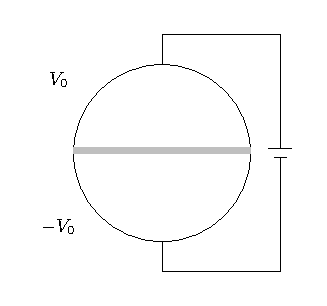
\includegraphics[scale=0.8]{Imagenes/Ejemplo_Esfera_03.eps}
\end{figure}
\end{frame}
\begin{frame}
\frametitle{Enunciado para los hemisferios con potencial}
Se nos pide calcular el valor del potencial en puntos exteriores a la esfera, es decir, para puntos tales que $r > a$.
\\
\bigskip
\pause
El problema sigue manteniendo una simetría azimutal, conocemos ya la expresión que nos determina la solución, solo debemos de tomar en cuenta la condición que establece el problema.
\end{frame}
\begin{frame}
\frametitle{Análisis de la solución general}
\begin{align*}
\Phi (r, \theta) = \sum_{k=0}^{\infty} \left( A_{k} \, r^{k} + \dfrac{B_{k}}{r^{k+1}} \right) \, P_{k} (\cos \theta)
\end{align*}
Los coeficientes $A_{k}$ deben de anularse ya que se espera que el potencial se cancele en el infinito. \pause
\\
\bigskip
Debiendo calcular entonces los coeficientes $B_{k}$.
\end{frame}
\begin{frame}
\frametitle{Otro caso con esferas}
Ahora consideremos el siguiente problema: Tenemos una esfera de radio $a$ formado por dos hemisferios a temperaturas $T_{1}$ y $-T_{1}$, éstos hemisferios están contenidos dentro de otra esfera de radio $b$, tal que $b > a$ y está a una temperatura $T_{2}$.
\end{frame}
\begin{frame}
\frametitle{Problema con dos esferas}
\begin{figure}
    \centering
    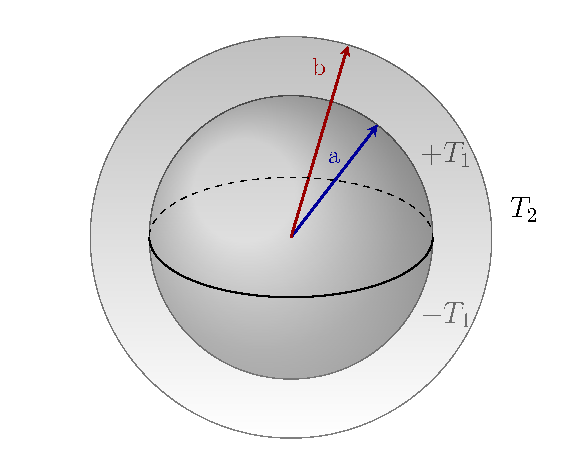
\includegraphics[scale=0.8]{Imagenes/Ejemplo_Esfera_02.eps}
\end{figure}
\end{frame}
\begin{frame}
\frametitle{Problema con dos esferas}
Se pide calcular la temperatura en:
\setbeamercolor{item projected}{bg=blue!70!black,fg=yellow}
\setbeamertemplate{enumerate items}[circle]
\begin{enumerate}[<+->]
\item Puntos interiores de la esfera de radio $a$: $r < a$.
\item Puntos entre la separación de las esferas: $a < r < b$.
\item Puntos exteriores de la esfera de radio $b$: $r > b$.
\end{enumerate}
\end{frame}
\begin{frame}
\frametitle{Resolviendo el ejercicio}
Ya sabemos como abordar la solución en el caso para puntos interiores de la esfera de radio $a$ y para puntos exteriores de la esfera de radio $b$.
\\
\bigskip
\pause
Para los puntos intermedios debemos de considerar las condiciones de continuidad que marca el ejercicio, de tal manera que en esta parte si será necesario considerar ambos coeficientes de la expresión $\Phi(r,\theta)$ que se dedujo.
\end{frame}
\end{document}